%\documentclass[12pt, letterpaper, titlepage]{article}
\documentclass[12pt, letterpaper]{article}

\usepackage{amsmath, amsfonts}
\usepackage{booktabs}
\usepackage{amsthm}
\usepackage{graphicx}
\usepackage[margin=1in]{geometry}
\usepackage{hyperref}
\usepackage{cleveref}
\hypersetup{colorlinks = true, linkcolor = blue, citecolor=blue, urlcolor = blue}
\usepackage{natbib}
\usepackage{float}
\usepackage{setspace}
\usepackage{pdfpages}
\usepackage{lineno}
\usepackage{mwe}
\usepackage{comment}
\linenumbers*[1]
% %% patches to make lineno work better with amsmath
\newcommand*\patchAmsMathEnvironmentForLineno[1]{%
 \expandafter\let\csname old#1\expandafter\endcsname\csname #1\endcsname
 \expandafter\let\csname oldend#1\expandafter\endcsname\csname end#1\endcsname
 \renewenvironment{#1}%
 {\linenomath\csname old#1\endcsname}%
 {\csname oldend#1\endcsname\endlinenomath}}%
\newcommand*\patchBothAmsMathEnvironmentsForLineno[1]{%
 \patchAmsMathEnvironmentForLineno{#1}%
 \patchAmsMathEnvironmentForLineno{#1*}}%

\AtBeginDocument{%
 \patchBothAmsMathEnvironmentsForLineno{equation}%
 \patchBothAmsMathEnvironmentsForLineno{align}%
 \patchBothAmsMathEnvironmentsForLineno{flalign}%
 \patchBothAmsMathEnvironmentsForLineno{alignat}%
 \patchBothAmsMathEnvironmentsForLineno{gather}%
 \patchBothAmsMathEnvironmentsForLineno{multline}%
}

% control floats
\renewcommand\floatpagefraction{.9}
\renewcommand\topfraction{.9}
\renewcommand\bottomfraction{.9}
\renewcommand\textfraction{.1}
\setcounter{totalnumber}{50}
\setcounter{topnumber}{50}
\setcounter{bottomnumber}{50}

\newcommand{\jy}[1]{\textcolor{blue}{JY: #1}}
\newcommand{\eds}[1]{\textcolor{red}{EDS: (#1)}}
\newcommand{\of}[1]{\textcolor{violet}{OF: #1}}

% NOTE: To produce blinded version, replace "0" with "1" below.
\newcommand{\blind}{0}

%\title{On Devon Allen's Disqualification at the 2022 World Track and Field
%Championships}
%
%\author{Owen Fiore\\
%%   \href{mailto:owen.fiore@uconn.edu}
%% {\nolinkurl{owen.fiore@uconn.edu}}\\
  %Elizabeth D. Schifano\\
  %Jun Yan\\[1ex]
  %Department of Statistics, University of Connecticut\\
%}
%\date{}

\begin{document}

\title{\bf On Devon Allen's Disqualification at the 2022 World Track and Field Championships}

\if0\blind
{
  \author{Owen Fiore, %\\
%   \href{mailto:owen.fiore@uconn.edu}
% {\nolinkurl{owen.fiore@uconn.edu}}\\
  Elizabeth D. Schifano, %\\
  Jun Yan\\[1ex]
  Department of Statistics, University of Connecticut\\
}
} \fi

\if1\blind
{
  \bigskip
  \bigskip
  \bigskip
  \author{Anonymous Authors}
  \bigskip
} \fi

\maketitle

\doublespace

% Abstract should be under 200 words

\begin{abstract}
Devon Allen’s disqualification at the men's 110-meter hurdle final at
the 2022 World Track and Field Championships, 
due to a reaction time (RT) of 0.099 seconds---just 0.001 seconds below
the allowable threshold---sparked widespread debate over 
the fairness and validity of RT rules. This study investigates two key
issues: variations in timing systems and the justification for the
0.1-second disqualification threshold. We
pooled RT data from men’s 110-meter hurdles and 100-meter dash, as
well as women’s 100-meter hurdles and 100-meter dash, spanning
national and international competitions. Using a rank-sum test for
clustered data, we compared RTs across multiple competitions,
while a generalized Gamma model with random effects for venue and heat
was applied to evaluate the threshold. Our analyses reveal significant
differences in RTs between the 2022 World Championships and other
competitions, pointing to systematic variations in timing
systems. Additionally, the model shows that RTs below 0.1 seconds,
though rare, are physiologically plausible. These findings highlight
the need for standardized timing protocols and a re-evaluation of the
0.1-second disqualification threshold to promote fairness in
elite competition.


\bigskip\noindent{\sc Keywords}:
false start, GAMLSS, reaction time, rank-based test, short sprint
\end{abstract}

\doublespace


\section{Introduction}
\label{sec:intro}

Devon Allen’s highly anticipated performance at the 2022 World
Track and Field Championships in Eugene, Oregon, ended in
controversy when he was disqualified for a reaction time (RT) of
0.099 seconds, just 0.001 seconds below the allowable threshold.
Allen, a University of Oregon alumnus,
had recently run a time of 12.84 seconds in the 110-meter hurdle
event, just 0.04 seconds short of the world record. After placing
third at the U.S. Track and Field Championships, he advanced
through the preliminary heats and semifinals at the World
Championships, with RTs of 0.123 and 0.101 seconds,
respectively. However, in the final heat, competing in front of his
home audience, Allen’s RT was just 0.001 seconds faster
than the 0.1-second threshold set by the International Association
of Athletics Federations (IAAF), resulting in his disqualification, a
decision that was met with widespread public outcry. This 
incident highlighted two long-standing issues: variability in the
measurement of RTs by Start Information Systems (SIS) and the
appropriateness of the 0.1-second disqualification threshold. As
reaction times are measured in fractions of a second, inconsistencies
in timing technologies and rules can significantly affect athlete
outcomes, raising questions about fairness and standardization.


World Athletics (formerly IAAF) uses certified SIS to measure RTs, yet
variation in technology persists. Discussions at online forums such as
\url{www.LetsRun.com} questioned consistencies in the SIS as a
contributing factor to RT anormalies \citep{johnson2022data,
  johnson2022was}. Historically, ``loud gun'' systems caused signal delays
for athletes in outer lanes  due to the speed of sound, an issue
addressed with the introduction of ``silent gun'' systems in 2010,
which electronically synchronize sound delivery to all athletes
\citep{tonnessen2013reaction}. Despite these advances, variability
persists due to differences in sensor technologies, such as force
transducers and accelerometers, and inconsistencies in event detection
algorithms \citep{willwacher2013novel}. For example, simple
force-threshold systems may delay RT detection by up to 26~ms compared
to more sophisticated methods \citep{pain2007sprint}. These findings
emphasize the need for standardized certification protocols to reduce
discrepancies and ensure fairness in RT measurements, as recently
reviewed by \citet{milloz2021sprint}.


Originally introduced in the 1990s to discourage athletes from attempting
to predict the start gun, the 0.1-second disqualification threshold 
has been the subject of significant debate.   Partly based on limited
data from Finnish national-level athletes~\citep{mero1990reaction}, the
threshold may not adequately represent the capabilities of elite
sprinters. Controlled experiments have shown that reaction times below
0.1 seconds are physiologically plausible \citep{pain2007sprint,
  komi2009iaaf}, while retrospective analyses of competition data
often advocate for raising the threshold~\citep{brosnan2017effects,
  lipps2011implications}. Stricter false-start rules, introduced to
minimize race disruptions, have also discouraged sprinters from
attempting faster starts, which may artificially inflate RTs recorded
in competition~\citep{haugen2013effect}. This divergence between
experimental findings and competition-based analyses illustrates the
complexity of defining a universally fair threshold. Addressing these
debates requires modern data collection and advanced methodologies to
ensure equity and consistency in elite
competition~\citep{milloz2021sprint}.


This paper addresses two primary objectives from a statistical
perspective, using modern methodologies to analyze historical
data. First, we investigate whether RTs at the 2022
World Championships were significantly different from other
competitions, focusing on athletes who competed in multiple
events. Using a matched-pairs design, we compare RTs across the 2022,
2019, and 2023 World Championships, as well as 2022 national-level
competitions. This approach isolates the effect of the competition
 while controlling for individual performance. The clustered
nature of the data, with the goal of assessing differences across
competitions within athletes, was analyzed using a rank-based comparison
approach for clustered data \citep{datta2005rank}. Second, we evaluate
the appropriateness of the 0.1-second disqualification threshold by
modeling RTs from World Championships held from 1999 onward. A
generalized Gamma (GG) distribution with random effects for both venue and
heat was applied within the framework of the generalized additive
model for location, scale, and shape (GAMLSS)
\citep{rigby2005generalized, stasinopoulos2024generalized}.
This model enables estimation of the
probability of RTs falling below a threshold, providing a
statistical assessment of RT consistency and the validity of the
current threshold.


%Needs to be looked at
The rest of this paper is organized as follows. Section~\ref{sec:problem1}
investigates RTs of athletes who competed at the 2022 World Championships to
examine differences between other competitions.  Section~\ref{sec:problem2}
investigates RTs of athletes from 1999 to 2023 to determine a reaction barrier
ground in statistical analysis.  Within each of the above sections, the data,
methods used, and the results are presented.
Finally, Section~\ref{sec:concludingremarks} highlights the
paper’s impact, limitations, and potential for future research.
All data and code for our analysis are provided in the Supplementary
Materials.

\section{Analysis of the 2022 World Championships RTs}
\label{sec:problem1}

\jy{State the hypotheses here before diving into data/methods/results.}
\of{Like this?  I feel like the first paragraph of the data section serves as
a good introductino to this section. I dont' know what to write without
re-writing the introduction or what is discussed in the first paragraph of 2.1}

This investigation began to determine whether athletes who competed at the 2022
Championships had significantly different RTs to when those same athletes
competed in comparable and relevant events. 

\of{or like this?}

Within our investigation to determine if athletes performed abnormally in 2022,
we will analysze times from athletes who competed in earlier meets in 2022 
or from another World Championship meet in 2019 or 2023.

\subsection{Data}
\label{sec:data_2022}


\jy{This two paragraphs are repetitive. Condense.}
\of{Resolved but needs to be proof read}
To investigate whether RTs at the 2022 World Championships
were significantly different from other competitions, we
used data from male athletes in the 110-meter hurdles and 100-meter
dash, and female athletes in the 100-meter hurdles and 100-meter dash,
provided they competed in the 2022 World Championships and at least
one other competition (2022 national championships, 2019 World
Championships, or 2023 World Championships). Statistical tests showed no
significant differences in RTs between these events, supporting their
inclusion in a unified analysis. However, we excluded data from
200-meter dashes and longer events, as their RTs were found
to be significantly different. This difference is not unexpected, as
RTs are generally less critical in longer sprint events
compared to shorter distances where explosive starts are paramount.
Negative RTs were excluded from the analysis, while positive disqualified RTs
were included due to their low frequency and not being obvious outliers.

  % A
% sensitivity analysis regarding the inclusion of positive disqualified
% RTs is provided in the Supplementary Material.




\subsubsection{2022 National Competitions}
\label{sec:datanational}

\jy{Opening sentence not accurate. This is the data to test the first
  hypothesis: national versus World Championship 2022.}
\of{Is it better now?}

%To assess the abnormality of the 2022 World Championships, we examined
%ata beyond World Championship events. This decision was motivated by

To determine if athletes reacted differently at the 2022 World Championships,
our first places that we look are 2022 national championships.
Prior to a formal analysis, we examined how United States (US) athletes
performed at the 2022 US Track and Field Championships, held from June 23--26,
2022, at Hayward Field in Eugene, Oregon. Since this venue also hosted
the 2022 World Championships in August, it
provided a unique opportunity to compare. There were four US
110-meter hurdle athletes—Trey Cunningham, Daniel Roberts,
Grant Holloway, and Devon Allen—who competed in both events. All four
athletes recorded faster RTs in every World Championships race
compared to their performances at the national-level event. Similarly,
all four US 100-meter dash athletes---Marvin Bracy, Fred Kerley,
Travyon Bromwell, and Christian Coleman---also recorded slower RTs at
the US Championships than at the World Championships.
To expand the dataset, we included RTs from 100-meter hurdle
and 100-meter dash athletes who competed in other national
competitions held between May and July 2022 across various
countries. Compiling this data presented challenges, as RTs were not
centrally archived and often required searching country-specific
websites, with many results recorded in native languages.


The final dataset consisted of RTs from athletes who competed
in both national and international competitions. RTs from
preliminary heats, semifinals, and finals were included to ensure
sufficient data for analysis. Excluding preliminary heats would have
significantly reduced the number of athletes and clusters. Each
athlete was considered as a cluster, with observed RTs
from both the `treatment' group (2022 World Championships) and
the `control' group (national competition) within the cluster. Cluster
sizes ranged from three to six, with a median size of four. Because gender
is known to influence RTs \citep{babicc2009reaction,
  lipps2011implications}, we prepared data for men and women
separately, resulting in 80 RTs from 17 athletes for each
gender. This setup forms the basis for the rank-based comparison for
clustered data with subunit-level grouping, which accounts for the
within-athlete dependence inherent in this data structure. The top
panel of Figure~\ref{fig:RankScatterplots} shows the RTs
of those who competed both at national competitions and the 2022 World
Championships.

\begin{figure}[tbp]
  \centering
  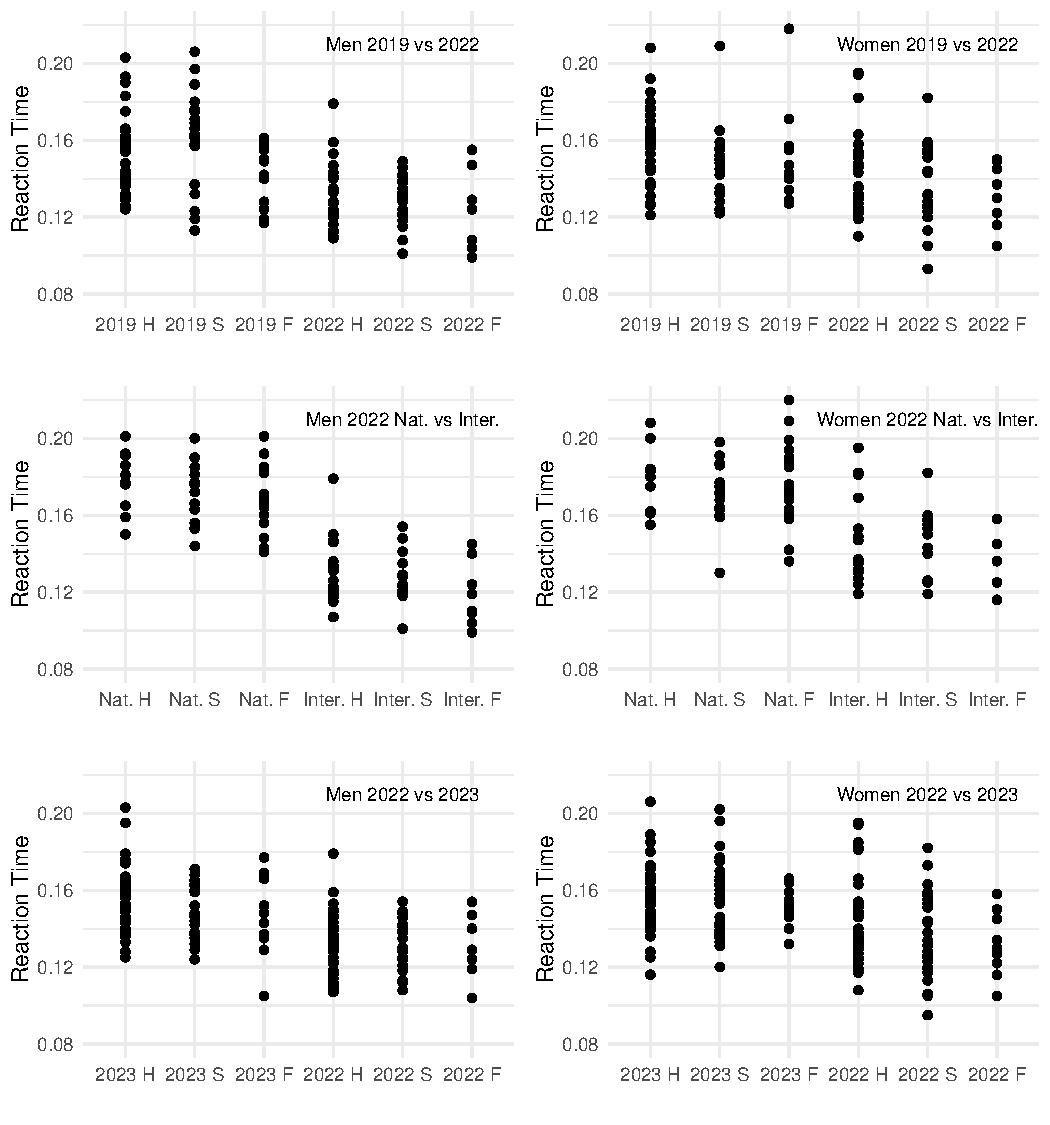
\includegraphics[width=\textwidth]{RankScatterPlots}
  \caption{RTs for athletes who competed at the 2022 World Championships
    and at another championship (2022 national, 2019 World, or 2023
    World) at which they competed. On the horizontal
    axis below each graph ``H'', ``S'', and ``F'' refer to the heats,
    semifinals, and  finals respectively. Please note that in the last
    row the 2022 times are to the right of the 2023 times.}
  \label{fig:RankScatterplots}
\end{figure}

\subsubsection{2019 and 2023 World Championships}
\label{sec:data2019}

\jy{Improve the topic sentence: this data is for the second
  hypothesis: 2019 vs 2022; 2023 vs 2022.}
\of{Is this more along the lines of what you are looking for}

This data was compiled to test our second focus, athletes who competed at
the 2022 World Championships and the 2019 or 2023 World Championships. 
In the 2019-2022 comparison,
RTs from 2022 were treated as the `treatment' group, with
2019 serving as the `control' group. Similarly, in the 2022-2023
comparison, RTs from 2022 were treated as the `treatment'
group, with 2023 serving as the `control' group. This structure allowed
us to prepare datasets suitable for examining RTs of athletes
who competed across multiple World Championships.


Each athlete was treated as a single cluster, containing their RTs
from different World Championships. The dataset for the 2019-2022
comparison contained 134 RTs from 34 male athletes and 124
RTs from 31 female athletes. The dataset for the 2022-2023
comparison contained 161 RTs from 45 male athletes and 182
RTs from 47 female athletes. While it is theoretically
possible that athletes improved their RTs between 2019 and
2022 or between 2022 and 2023, such improvements are highly unlikely for
elite sprinters, as they already operate near the limits of human
performance. Consequently, consistent improvements observed in 2022
would suggest systematic differences rather than natural variability.


Figure~\ref{fig:RankScatterplots} shows the RTs of athletes
who competed in both the 2019 and 2022 World Championships (middle
panel) and those who competed in both the 2022 and 2023 World
Championships (lower panel). The athletes included in the 2022 data
differ between these two comparisons, as the set of athletes who
competed in both 2019 and 2022 is not the same as the set who competed
in both 2022 and 2023. To be included, athletes must have competed in
at least one race at each championship. Notably, Devon Allen recorded
the fastest RTs in both the Finals and Semifinals of the
2022 World Championships, but his disqualification was determined by a
difference of just 0.002 seconds, with RTs of 0.101 and
0.099 seconds, respectively. This highlights the critical role of
RT precision in elite-level competition.

\subsection{Methods}
\label{sec:methods_2022}


To test the conjecture that the 2022 World Championships timing device may have
led to faster recorded RTs, we compare the RTs of the same
athletes who have attended both the 2022 World Championships and other
competitions.
In this setting, we have clustered data with subunit grouping. In particular,
each athlete is a cluster and the multiple RTs from the same athlete
can be from either the 2022 World Championships or otherwise.
Let $X_{ij}$ be the $j$th RT of athlete~$i$, $i = 1, \ldots, n$,
$j = 1, \ldots, m_i$ where $m_i$ is the number of observations from
athlete~$i$. Let $\delta_{ij}$ be the group indicator of $X_{ij}$; $\delta_{ij}
= 1$ if $X_{ij}$ is in group~1 (2022 World Championships) and $\delta_{ij} = 0$
otherwise. Athletes are
assumed to be independent, while subunit observations from the same athlete are
not. The null hypothesis $H_0$ to be tested is that there is no difference
between the two groups; i.e., the distribution of $X_{ij}$ remains the same
regardless of the group indicator $\delta_{ij}$.


\citet{datta2005rank} proposed an extension of the Wilcoxon rank-sum test to
clustered data with subunit-level grouping. The test is designed based on a
within-cluster resampling principle. Consider randomly picking one observation
from each cluster to form a pseudo-sample. Let $X_i^*$ be a random pick from the
$i$th cluster in the pseudo-sample and $\delta_i^*$ its group indicator. The
Wilcoxon rank-sum statistic for the pseudo-sample is
\[
W^* = \frac{1}{n + 1} + \sum_{i=1}^{n} \delta_{i}^{*} R_{i}^{*},
\]
where $R_{i}^{*}$ is the rank of $X_{i}^{*}$ in the pseudo-sample.
The test statistic $S$ is the average of $W^*$, averaged over all possible
pseudo-samples conditioning on the observed data and group indicators.
The mean and variance of $S$ under $H_0$ can be derived so that $S$ can be
standardized to form a $Z$ statistic which follows a standard normal distribution
asymptotically \citep[p.910]{datta2005rank}.


When the sample size is small, the asymptotic normal distribution may
not be reliable, so we also use 1~million random permutations to
simulate the null distribution of the test statistic.
This method is available from the \texttt{clusWilcox.test()} function
with \texttt{method = `ds'} (for \underline{D}atta and \underline{S}atten) and
\texttt{exact = TRUE} from R package
\texttt{clusrank} \citep{jiang2020wilcoxon}.


\subsection{Results}
\label{sec:results_2022}


The rank-based methods described in Section~\ref{sec:methods_2022} were used to
compare RTs between the 2022 World Championships and other
competitions in which the same athletes participated. These comparisons
were conducted separately for men and women, resulting in six total
comparisons: RTs from the 2022 national-level championships
versus the 2022 World Championships for men and women, RTs
from the 2019 versus 2022 World Championships for men and women, and
RTs from the 2022 versus 2023 World Championships for men and
women.


\begin{table}
  \centering
  \caption{P-values of comparisons between
    RTs from different competitions for the same athletes.
    2022 Nat. vs Inter. compares RTs from 2022 national-level
    championships and the 2022 World Track and Field Championships. 2019
    vs 2022 compares RTs from the 2019 and 2022 World Track and
    Field Championships. 2022 vs 2023 compares RTs from the
    2022 and 2023 World Track and Field Championships.}
  \begin{tabular}{c c c c c}
   \toprule
   Comparison & Permutation & Asymptotic & \# of athletes & \# RTs  \\
   \midrule
   2022 Nat. vs Inter. Men & $1.0 \cdot 10^{-6}$ & $ 6.1 \cdot 10^{-5}$ & 17 & 80 \\
   2022 Nat. vs Inter. Women & $1.0 \cdot 10^{-6}$ & $ 1.2 \cdot 10^{-3}$ & 17 & 80 \\[1ex]
   2019 vs 2022 Men & $2.8 \cdot 10^{-5}$ & $1.1 \cdot 10^{-5}$ & 34 & 134 \\
   2019 vs 2022 Women & $ 1.5 \cdot 10^{-3}$ & $6.9 \cdot 10^{-3}$ & 31 & 124 \\[1ex]
   2022 vs 2023 Men & $1.0 \cdot 10^{-6}$ & $1.4 \cdot 10^{-6}$ & 45 & 161 \\
   2022 vs 2023 Women & $1.0 \cdot 10^{-6}$ & $9.4 \cdot 10^{-7}$ & 47 & 182 \\
   \bottomrule
  \end{tabular}
  \label{tab:Clusrankresults}
\end{table}


Table~\ref{tab:Clusrankresults} presents the results from both permutation
and asymptotic rank-based tests for the six comparisons. All tests
yielded very small p-values, even after applying a Bonferroni
adjustment for multiple comparisons, indicating consistent evidence of
faster RTs at the 2022 World Championships relative to other
competitions. For both men and women, the national versus
international comparisons showed that RTs at the 2022 World
Championships were significantly faster than at national-level
competitions held earlier that year. Similarly, comparisons between
the 2019 and 2022 World Championships and between the 2022 and 2023
World Championships produced significant results, reinforcing the
observation that RTs at the 2022 World Championships were notably
faster. These findings support the hypothesis that conditions at the
2022 World Championships, whether systematic or
environmental, contributed to consistently faster RTs.


We also conducted the same analysis with men’s and women’s data
pooled, yielding similar results. Details are provided in Section~1 of
the Supplementary Material.

\section{Analysis of the 0.1 RT Barrier}
\label{sec:problem2}

\jy{write a quick overview paragraph here.}
\of{Is it too much of a re-telling of the introduction?}

In addition to the work presented in Section~\ref{sec:problem1} we thought that
it was relevant and important to expand on prior work that focused on an
appropriate reaction time barrier.  Implemented by World Athletics to discourage
false starts, athletes with RTs below 0.1 seconds are disqualified.  In this
section we will attempt to model historical data to recommend a reaction barrier
based in statistical analysis.


\subsection{Data}
\label{sec:data_barrier}

The data for evaluating the appropriateness of the 0.1-second
threshold was obtained from World Athletics and covers the men's
110-meter hurdles and 100-meter dashes from 1999 to 2023. Due to
possible gender differences \citep{babicc2009reaction,
  lipps2011implications}, data for women's 100-meter hurdles and
100-meter dashes and their analyses were relegated to the
Supplementary Material. We focus on the RTs recorded during
semifinal and final heats only, as RTs from preliminary
heats are often not as fast as those in later heats
\citep[e.g.,][]{collet1999strategic, tonnessen2013reaction,
  brosnan2017effects, zhang2021correlation}. For analysis purposes, we
pooled RTs from semifinal and final heats to increase sample
size, which is particularly important for years with limited final heat
observations. For example, in 2022, only five data points were available
from the final heat due to two disqualifications and one athlete not
competing. Unless otherwise noted, this pooled dataset forms the basis
for our analyses for Objective 2. Additionally, we consider datasets
that exclude 2022 to assess how our findings might differ when excluding
this year of interest. This investigation began shortly after the 2022 World
Championships, and we were pleased that including data from 2023 did not
significantly alter our results \citep{WAData}.  


The data is summarized in Figure~\ref{fig:Boxplot}, which presents a
sequence of boxplots of RTs from 1999 to 2023. It is evident
that RTs in 2022 were notably faster, with a median reaction
time of 0.129 seconds compared to the 0.156 seconds observed in earlier
studies, such as \citet{brosnan2017effects} for data spanning 1999 to 2014.
Figure~\ref{fig:Boxplot} also highlights year-to-year variability in
RTs, likely influenced by changes in the championship venue
and environmental conditions such as humidity, precipitation, and
elevation. Furthermore, advancements in technology and alterations to
false start rules during the study period may have played a role in these
variations \citep{willwacher2013novel}.


\begin{figure}[tbp]
  \centering
  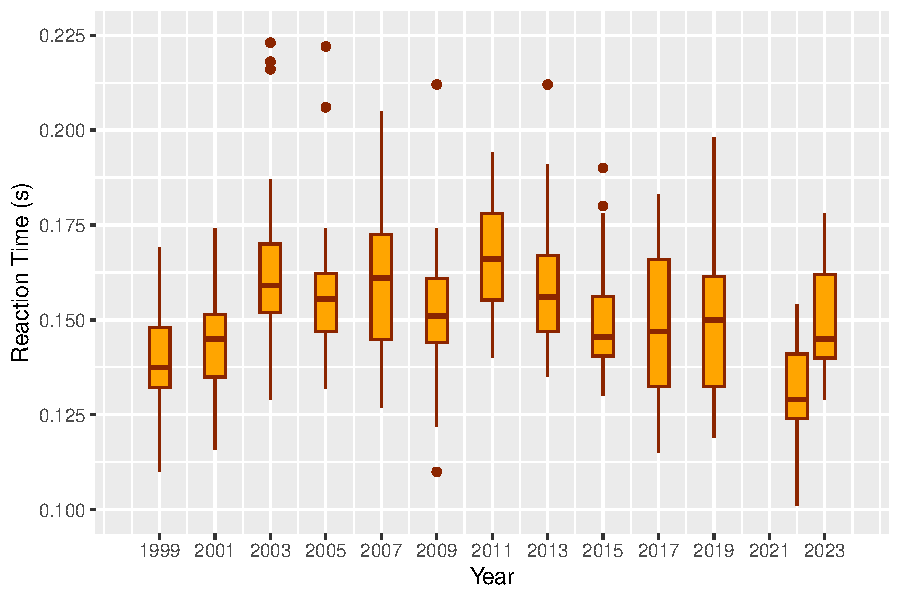
\includegraphics[width=\textwidth]{Boxplot}
  \caption{The RTs from 1999 to 2023 for the men's 110 meter hurdle
  and 100 meter dash.}
  \label{fig:Boxplot}
\end{figure}


Between 2007 and 2009, World Athletics allowed one
false start warning before disqualifying a sprinter \citep{iaaf2009falsestart}.
This lenient rule led to 18 male and 7 female false starts at both the 2007
and 2009 World Championships. In 2011, this rule was replaced with the stricter
policy of automatic disqualification for false starts, aimed at reducing the
delays caused by repeated warnings. This change reduced men’s false starts
by two-thirds in 2011, with only six male and four female disqualifications
\citep{iaaf2009falsestart}. \citet{haugen2013effect} demonstrated that more
lenient false start rules significantly improved RTs during the
1997–2009 period, suggesting that rule changes over the study period may
have contributed to variations in RTs across years.


\subsection{Methods}
\label{sec:methods_barrier}


Based on an exploratory analysis, the RTs are adequately
modeled by a GG distribution with random effects in
model parameters. The GG distribution has three parameters, denoted by
$\text{GG}(\mu, \sigma, \nu),$ has density function
\begin{equation}
  \label{eq:gg}
f_Y(y \mid \mu, \sigma, \nu) =
\frac{|\nu| \theta^\theta z^{\theta}}{\Gamma(\theta) y}
\exp\left(-z \theta\right),
\end{equation}
for $y > 0$, $\mu > 0$, $\sigma > 0$, and $\nu \neq 0$,
where $z = (y / \mu)^\nu$,
$\theta = 1 / (\sigma^2 \nu^2)$, and
$\Gamma(\cdot)$ denotes the Gamma function.
The GG distribution is highly flexible, encompassing several
well-known distributions as special cases, such as the
Weibull ($\mu = \nu)$ and  Gamma $(\nu = 1)$ distributions.
Its expectation is
\[
  \frac{\mu \Gamma(\theta + 1 / \nu)}
  {\theta^{1 / \nu} \Gamma(\theta)},
\]
provided $\theta > -1 / \nu$. Here,
$\mu$ scales the central tendency, $\sigma$ controls
dispersion, and $\nu$ determines skewness. This parameterization allows
the distribution to model asymmetric and heavy-tailed data effectively, making
it particularly suitable for RTs.
An implementation of this distribution is available from R package
\texttt{gamlss.dist} \citep{rigby2019distributions}.


Random effects at the venue and heat levels are incorporated to the
parameters in GG distribution in~\eqref{eq:gg}.
Let $Y_{ijk}$ denote the RT of observation~$k$ in heat~$j$
of year~$i$. Conditioning on a venue effect $v_i$ for year~$i$
and a heat effect $h_{i/j}$ nested within each year~$i$, the
distribution of $Y_{ijk}$ is
$\text{GG}(\mu_{ijk}, \sigma_{ijk}, \nu)$, where
\begin{align}
\log(\mu_{ijk}) &= \beta_0 + v_i , \label{eq:mu}\\
\log(\sigma_{ijk}) &= \gamma_0 + h_{i/j} , \label{eq:sigma}
\end{align}
$v_i$ is normally distributed with mean zero and
variance~$\tau_v^2$, and $h_{i/j}$ is normally distributed with mean
zero and variance~$\tau_h^2$.
The two random effects were found useful: one 
capturing the venue effect, which is used to contrast years, and the 
second being the heat effect, where every race was given a unique 
identifier with typically five to nine observations per race.
This model can be fit with R package \texttt{gamlss} 
\citep{stasinopoulos2008generalized}. The heat effect could be added
to the model for $\mu_{ijk}$ and the venue effect could be added to 
the model for $\sigma_{ijk}$. From our comparison using the Akaike 
Information Criterion, Models~\eqref{eq:mu}--\eqref{eq:sigma} turned 
out to be preferred to more complex models or competing models.


Model diagnosis and tail analysis can be done with the fitted GG model
from package \texttt{gamlss}. Normalized quantile residuals, or
z-scores \citep{dunn1996randomized}, of the observations can be
extracted with the \texttt{residuals} method of a \texttt{gamlss}
object. The z-scores can then be checked with a Q-Q plot
\citep{almeida2018ggplot2}. The marginal
distribution of $Y_{ijk}$ is a scale-mixture of GG distributions, which can be
easily simulated from once the parameters are estimated. Many
random numbers generated from the fitted mixture distribution can be used to
approximate the probability of observing a RT faster than any given
threshold. We are specifically interested in the probability of a RT
being less than 0.1 seconds in order to gauge if that is a reasonable
disqualification barrier.



\subsection{Results}
\label{sec:results_barrier}

The results reported in this subsection are from men's data only
because our investigation found significant gender difference.
Results for women's data are reported in Section~2 of the
Supplementary Material. The fitted parameters of the GG distribution in the
GAMLSS framework in Equations~\eqref{eq:gg}--\eqref{eq:sigma} are
summarized in Table~\ref{tab:ggfit}. Results obtained from both
excluding and including 2022 data are reported. The fixed-effect
parameters include $\beta_0$, $\gamma_0$, and $\nu$, corresponding to
the intercept of the log-location, log-scale, and shape of the GG
distribution, respectively. Random effects account for variability at
the venue level on the log-scale of the $\mu$ parameter
and at the heat level on the log-scale of the $\sigma$
parameter in the density in Equation~\eqref{eq:gg}. The variance
of the venue-level random effect is smaller than the heat-level random
effect variance, suggesting that heat-level variability in the scale
parameter is substantial, though on the dispersion parameter. When the
2022 data is included, all parameter estimates remain stable except
the standard deviation of the venue-level random-effect,
which increases from 0.043 to 0.058. These results
highlight that RTs are influenced by both venue and heat-level
factors, and that the inclusion of 2022 introduces greater venue-level
variability, likely due to systematic differences in RTs that year.


\begin{table}
  \centering
  \caption{Estimated fixed-effect parameters with standard errors in
    parentheses and estimated standard deviations of the random effects from the
    fitted GG distribution with venue level random
    effects in $\mu$ and heat level random effects in $\sigma$ in
    Models~\eqref{eq:gg}--\eqref{eq:sigma}.}
  \label{tab:ggfit}
  \begin{tabular}{c c c c c c}
    \toprule
    Data set & $\beta_0$ & $\gamma_0$ & $\nu$ & $\tau_v$ & $\tau_h$ \\
    \midrule
    Excluding 2022 & $-$1.910 (0.005) & $-$2.200 (0.025) & $-$1.177 (0.442) & 0.043 & 0.326 \\
    Including 2022 & $-$1.910 (0.005) & $-$2.200 (0.027) & $-$1.178 (0.447) & 0.058 & 0.320 \\
    \bottomrule
  \end{tabular}
\end{table}

\begin{figure}[tbp]
  \centering
  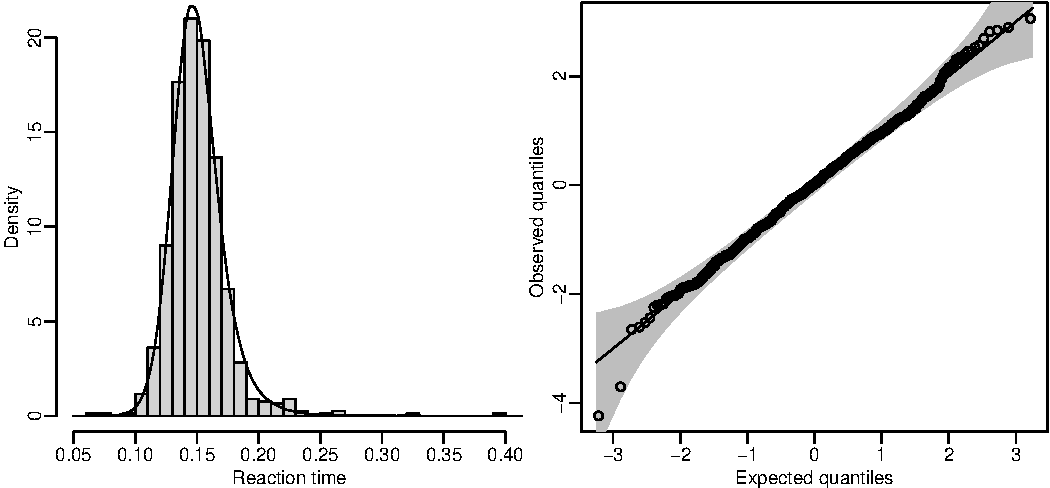
\includegraphics[width=\textwidth]{diagnosis.pdf}
  \caption{Diagnosis of the fitted GG distribution with
    random effects in model parameters: kernel density of 1 million
    observations drawn from the fitted model overlaid with the
    histogram of the observed RTs (left); Q-Q plot of the
    normal z-score of the quantile residuals from the fitted model (right).}
  \label{fig:diagnosis}
\end{figure}


Figure~\ref{fig:diagnosis} presents diagnostic checks for the fitted
GG distribution model with random effects. The left
panel compares the kernel density estimate of one million simulated reaction
times from the fitted model to the histogram of the observed RTs.
The close alignment between the density curve and the histogram suggests that
the fitted GG model adequately captures the overall distribution of the
RTs. The right panel shows a Q-Q plot of the z-scores of the
quantile residuals from the fitted model. The points lie approximately along
the 45-degree reference line, indicating that the residuals are consistent
with the standard normal distribution, supporting the adequacy of the model
fit. These diagnostics collectively demonstrate that the fitted model provides
a reasonable representation of the observed RT data.


\begin{table}
  \centering
  \caption{Probabilities of observing RTs less than threshold 0.08,
  0.09, and 0.10 seconds based on the
    fitted GG GAMLSS model with both venue- and heat-level
random effects.}
  \begin{tabular}{c c c c}
   \toprule
   Data Set & Threshold 0.08 & Threshold 0.09 & Threshold 0.10  \\
   \midrule
   Excluding 2022 & $5.31\cdot10^{-5}$ & $3.53\cdot10^{-4}$ &  $1.94\cdot10^{-3}$  \\
   Including 2022 & $6.84\cdot10^{-5}$ & $4.95\cdot10^{-4}$ & $2.76\cdot10^{-3}$ \\
   \bottomrule
  \end{tabular}
  \label{tab:Sim_probability}
\end{table}


The fitted GG GAMLSS model with both venue- and heat-level
random effects provides a framework for assessing how extreme RTs
below certain thresholds are. The probability of observing a RT
below a given threshold, assuming no intentional false starts, was approximated
by generating 10 million realizations from the fitted model.
Table~\ref{tab:Sim_probability} summarizes the probabilities of observing
RTs below 0.08, 0.09, and 0.10 seconds under two scenarios: one
excluding and the other including data from 2022. Excluding 2022 slightly
reduces the probability of observing a fast RT, but the difference
is small. For example, the probability of a RT below 0.10 seconds
decreases from $2.76 \cdot 10^{-3}$ (approximately one in 362 starts) to
$1.94 \cdot 10^{-3}$ (approximately one in 515 starts) when 2022 is excluded.
Lowering the RT threshold from 0.10 to 0.08 seconds drastically
reduces the likelihood of observing a RT below the barrier, with
the probability dropping from one in every 362 starts (at 0.10 seconds) to one
in every 14620 starts (at 0.09 seconds) and one in every 146198 starts (at 0.08
seconds) when 2022 is included. These results highlight the rarity of extremely
fast RTs and substantiate the recommendations of \citet{komi2009iaaf}
to carefully consider the selection of RT thresholds.


\begin{table}
  \centering
  \caption{Suggested RT barriers based on tail probabilities.}
  \begin{tabular}{c c c c}
   \toprule
   Data Set & Tail probability  $10^{-2}$ & Tail probability  $10^{-3}$ & Tail probability $10^{-4}$ \\
   \midrule
   Excluding 2022 & $0.111$ & $0.096$ & $0.083$ \\
   Including 2022 & $0.108$ & $0.094$ & $0.082$ \\
   \bottomrule
  \end{tabular}
  \label{tab:Sim_time}
\end{table}

Utilizing the same model, we can determine suitable RT barriers
based on the probability of observing a time below the barrier. As shown in
Table~\ref{tab:Sim_time}, including the 2022 data suggests a RT
barrier of 0.094 seconds to maintain a 0.1\% chance of observing an
exceptionally fast RT, while a stricter threshold of 0.082 seconds
is needed to limit this probability to 0.01\%. Excluding the 2022 data results
in slightly higher thresholds of 0.096 and 0.083 seconds for the respective
probability levels. These results indicate that while the inclusion of 2022
data slightly reduces the recommended barrier, the magnitude of the difference
is relatively small. This approach allows for tailoring RT
thresholds to desired levels of false positive rates, balancing fairness and
precision in disqualification criteria.




\section{Discussion}\label{sec:concludingremarks}


This study first examined whether reaction times (RTs) at the 2022
World Track and Field Championships were significantly faster than at
other competitions. Our analyses indicate that RTs at the 2022 World
Championships were consistently faster than those recorded at both
national-level competitions earlier in the same year and the 2019 and
2023 World Championships. The persistence of this pattern across
different comparison groups suggests that these differences are not
due to random variation or individual improvements over time. A more
comprehensive analysis would benefit from a centralized database
containing RTs from all World Athletics-certified meets, but such data
are not consistently available. However, by incorporating competitions
from multiple years (2019, 2022, and 2023), the analysis accounts for
potential confounding factors such as seasonality and age, as athletes
at different stages of their careers are represented in different
comparisons.


This study further assessed whether the 0.1-second RT threshold is a
fair standard for disqualification. Our analyses of the GAMLSS model
suggest that while RTs below 0.1 seconds are rare, they may not be
be as extraordinary as traditionally assumed. For men,
Table~\ref{tab:Sim_time} shows that RTs below 0.1 seconds
occur with a probability of approximately one in 362 starts when
including the 2022 data. Lowering the threshold to 0.08 seconds
drastically reduces this likelihood, supporting the idea that the
current barrier could be adjusted to reflect more realistic
probabilities of false starts. A similar pattern is observed for
women, as detailed in the Supplementary Material, where RTs
 below 0.1 seconds are exceedingly rare for the 100-meter dash
and 100-meter  hurdles. However, the uniformity of the 0.1-second
barrier for both men and women  is questionable, given numerous
studies documenting gender differences in reaction  times
\citep[e.g.,][]{lipps2011implications, babicc2009reaction,
  panoutsakopoulos2020gender}. These studies suggest that the current
threshold may  unfairly penalize men, for whom sub-0.1-second reaction
times are more probable. \citet{brosnan2017effects} advocate for
gender-specific barriers, a position that  aligns with our findings
and highlights the importance of tailoring thresholds to biological
distinctions.


This study provides a statistical framework to examine Devon Allen’s
disqualification at the 2022 World Track and Field Championships,
offering insights rather than drawing definitive conclusions about
potential equipment malfunction. Our findings indicate that RTs
 at the 2022 World Championships were, on average, faster than at other
competitions, as evidenced by the significant p-values in
Table~\ref{tab:Clusrankresults}. Additionally, the GAMLSS results
suggest that the 0.1-second barrier may not be as stringent as
previously believed. Based on Table~\ref{tab:Sim_time}, a stricter
threshold of 0.08 seconds could be considered, allowing athletes like
Allen to react swiftly without undue risk of disqualification. While
this analysis provides a rigorous statistical perspective, it does not
consider biomechanical factors, such as individual variability in
neuromuscular response times or the role of starting block sensors in
detecting pressure changes, which may offer more direct evidence of
reaction capabilities. In summary, while the results designate 2022 as
an anomalous year, Allen’s time, despite resulting in
disqualification, may not be categorically extreme.


\section*{Supplementary Material}
Additional results are summarized in a supplement for (1) rank-based
comparison with pooled (men and women) data, (2) GAMLSS results
for women's data, and (3) sensitivity of including positive yet disqualified
reaction times in GAMLSS.
The data and R code used for the analysis are available in a compressed file for
ease of reproducibility.

\bibliographystyle{apalike}
\bibliography{citations}


\end{document}
